\chapter{Supplement to Chapter~\ref{art}}\label{app.art}
%===================================================================================================
\section{Objective~1}\label{app.art.1}
%---------------------------------------------------------------------------------------------------
\subsection{Scenario Cascades}\label{app.art.1.cascade}
Figure~\ref{fig:art.1.cascade} illustrates cascade attainment over time across
the base case and ``who is left behind'' counterfactual scenarios (Table~\ref{tab:art.scenarios})
for FSW, clients, everyone else, and the population overall.
Transient declines in VLS among treated around 2010 correspond to expanding ART eligibility.
\begin{figure}[h]
  \centerline{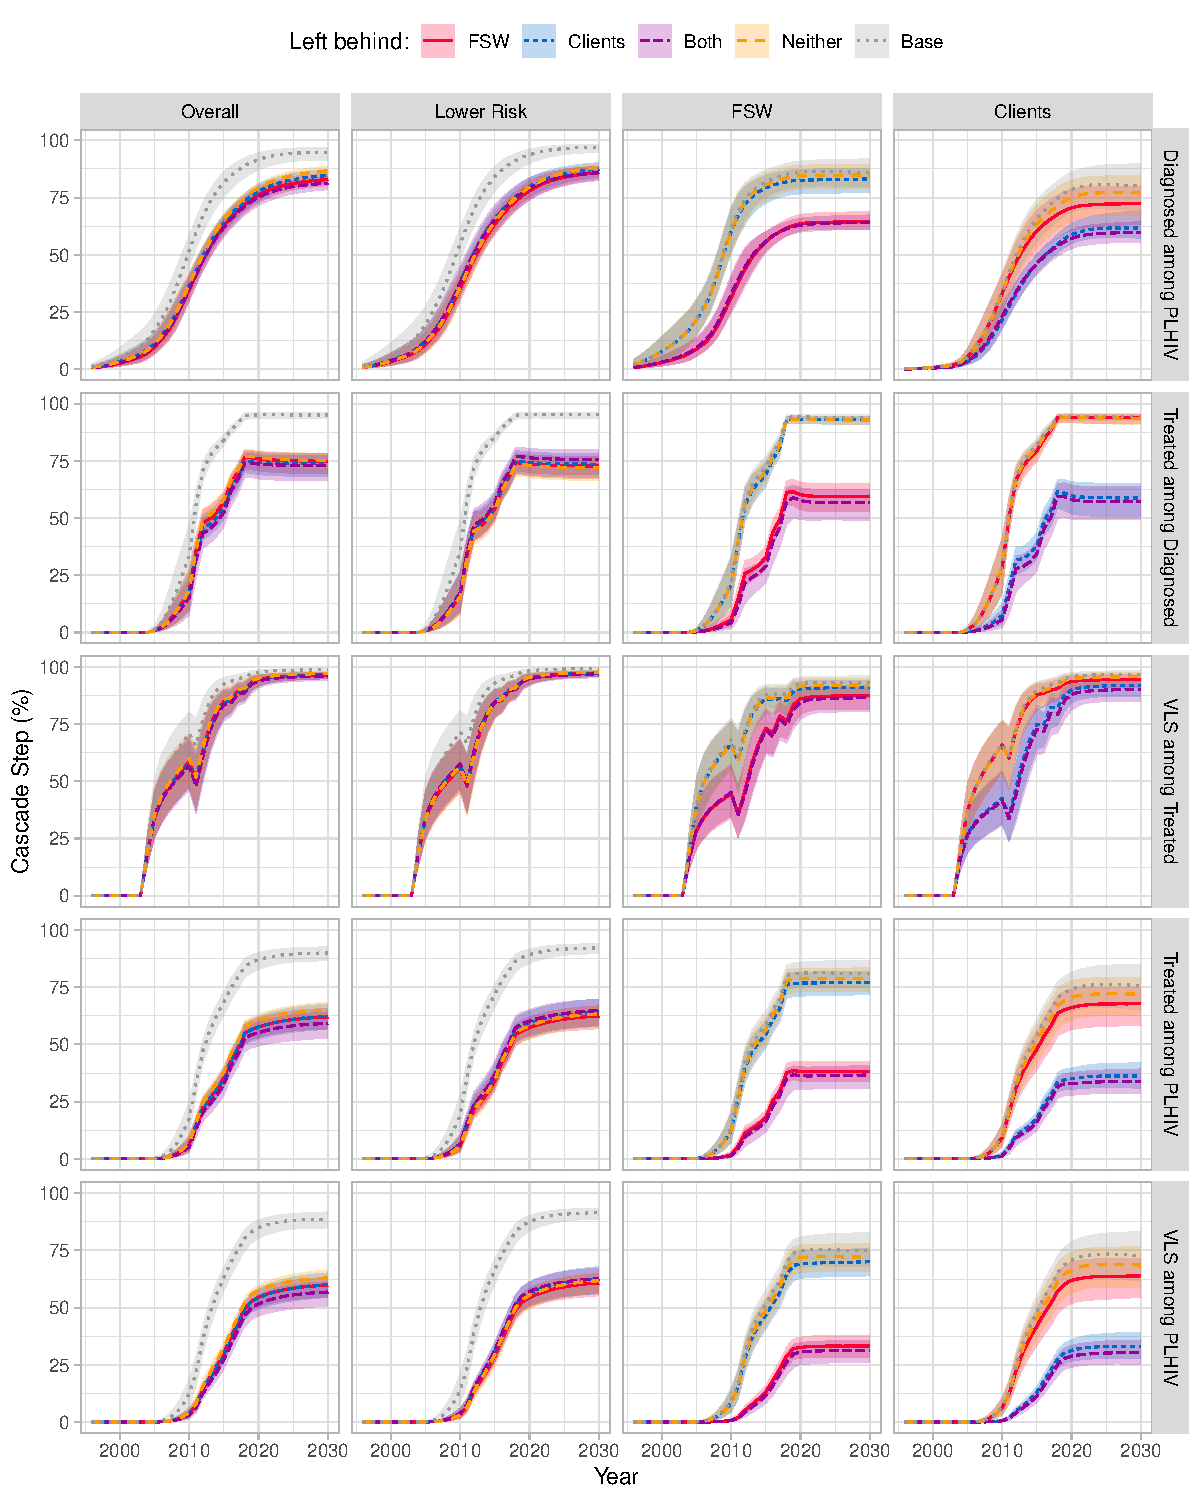
\includegraphics[scale=.8]{art.1.cascade}}
  \caption{Cascade attainment over time across scenarios}
  \label{fig:art.1.cascade}
  \floatfoot{\ffpopz; \ffcas; \ffart; \ffribbon.}
\end{figure}
%---------------------------------------------------------------------------------------------------
\subsection{Distributions of Additional Infections}\label{app.art.1.wiw}
As in \sref{model.res.wiw}, Figure~\ref{fig:art.1.wiw} illustrates
the distributions of additional infections over time \vs the base case across
``who is left behind'' counterfactual scenarios  (Table~\ref{tab:art.scenarios}),
stratified by partnership type, transmitting group, and acquiring group.
\begin{figure}
  \subcapoverlap
  \foreach \var in {part,from,to}{
  \begin{subfigure}{\linewidth}
    \includegraphics[width=\linewidth]{art.1.wiw.\var}
    \caption{\raggedright}
    \label{fig:art.1.wiw.\var}
  \end{subfigure}}
  \caption{Additional infections in each ``who is left behind'' counterfactual scenario
    \vs the base case, stratified by:
    \sfref{fig:art.1.wiw.part} partnership type,
    \sfref{fig:art.1.wiw.from} transmitting group, and
    \sfref{fig:art.1.wiw.to} acquiring group}
  \label{fig:art.1.wiw}
  \floatfoot{\ffart; \ffwiw.}
\end{figure}
%===================================================================================================
\section{Objective~2}\label{app.art.2}
Figure~\ref{fig:art.2.cascade} illustrates the distributions of cascade attainment by 2020
for FSW, clients, everyone else, and the population overall,
in the 10,000 randomly generated counterfactual scenarios
for the Objective~\ref{obj:art.2} regression analysis.
\begin{figure}[h]
  \centering
  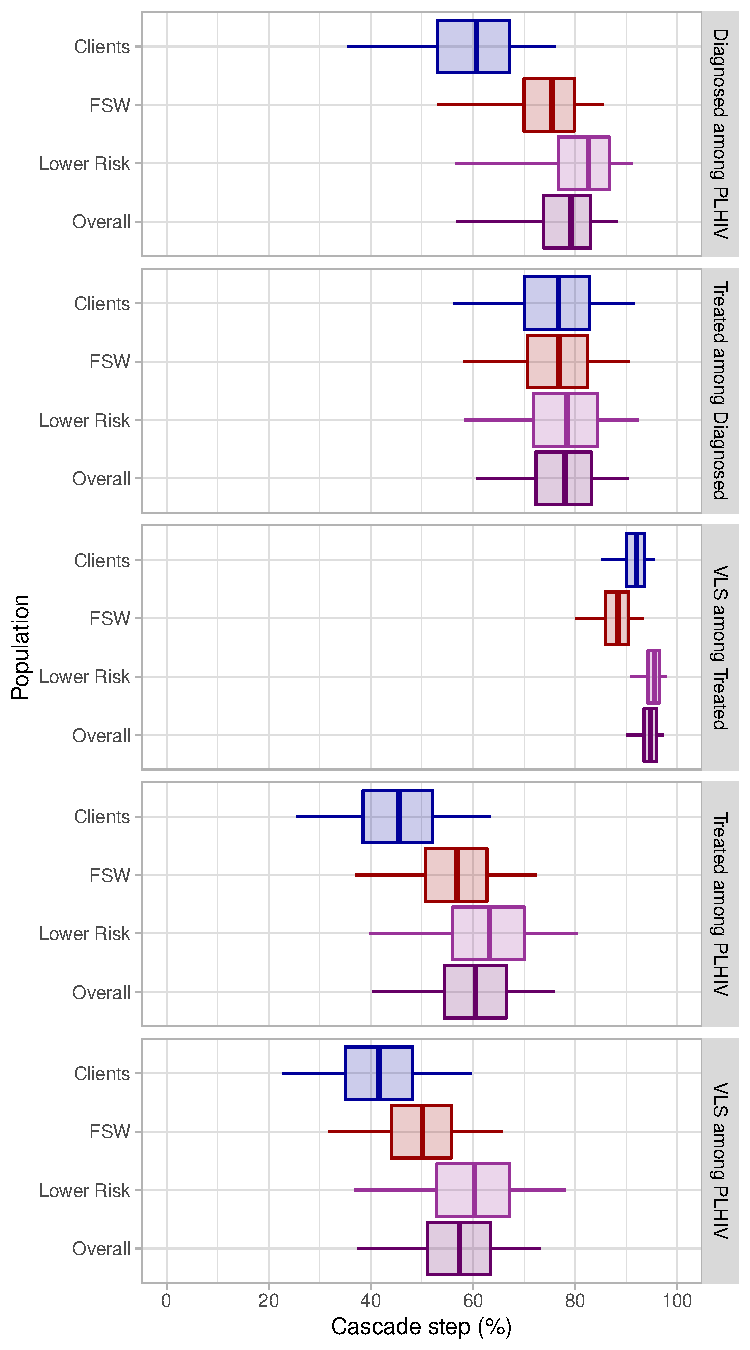
\includegraphics[scale=.8]{art.2.cascade}
  \caption{Cascade attainment by 2020 across 10,000 randomly generated counterfactual scenarios}
  \label{fig:art.2.cascade}
  \floatfoot{\ffpopz; \ffcas; \ffbox.}
\end{figure}
\printchapterbibliography
